% 2012/09/10 [Greetje] Enkele opmerkingen toegevoegd nav versie 5.4; enkele oefeningen over grafieken toegevoegd
% 2012/09/06 [Greetje] label toegevoegd voor hoofdstuk
% 19/02/2012 [Jan]: Oefeningen hernummerd met begin{oef} enz. Tabellen iets opgefrist, fouten 
%verbeterd

\chapter{Beknopte handleiding Scilab}
\label{scilab}
\begin{quote}
     \textit{{\small `Ik heb de das gekregen', vervolgde Wiggel 
Waggel nadenkend, terwijl hij de ene knie over de andere sloeg en 
zijn handen eromheen vouwde, `ik heb hem gekregen ---als 
onverjaardagscadeau'}}

     \textit{{\small `Pardon?' zei Alice met een verbluft gezicht.}}

     \textit{{\small `Ik ben niet beledigd,' zei Wiggel Waggel.}}

     \textit{{\small `Ik bedoel, wat is een onverjaardagscadeau?'}}
     \textit{{\small `Een cadeau gegeven wanneer het niet je verjaardag is, natuurlijk.'}}
	\textit{{\small Alice dacht even na. `Ik hou het meest van verjaardagscadeaus,' zei ze tenslotte.}}
	
	
\textit{{\small `Je weet niet waar je het over hebt!' riep wiggel 
Waggel. `Hoeveel dagen zitten er in een jaar?'}}
	
	\textit{{\small 
`Driehonderdvijfenzestig,' zei Alice.}}
			
	\textit{{\small `En 
hoeveel verjaardagen heb je?'}}
	
	\textit{{\small `E\'{e}n.'}}
	
	
\textit{{\small `En als je \'{e}\'{e}n aftrekt van 
driehonderdvijfenzestig, wat blijft er dan over?'}}
	
	
\textit{{\small `Driehonderdvierenzestig natuurlijk.'}}
	
		
\textit{{\small Wiggel Waggel leek te weifelen. `Dat zie ik liever 
even op papier,' zei hij.}}
		
          Uit `Achter de spiegel' -- Lewis Carroll
\end{quote}

\newpage

\section{Inleiding}

Het (freeware)-pakket Scilab\footnote{Download en documentatie op www.scilab.org.} is geschikt om numerieke problemen op te lossen. Het beschikt daarvoor over een omvangrijke ingebouwde functieset. Je kan deze set uitbreiden en aanpassen aan je eigen behoeften door gebruik te maken van de programmeermogelijkheid die Scilab biedt.

De aangewezen  manier om te leren programmeren in Scilab is experimenteren en voorbeelden bekijken (\texttt{.sci} en \texttt{.sce} bestanden).

Op \url{http://www.scilab.org/support/documentation/} vind je volledige documentatie. In het bijzonder raden we de documentatie onder het item `Tutorials' aan.  Verder heeft Scilab een goed uitgebouwde helpfunctie. Typ \verb+help+ in de commandolijn en het helpvenster verschijnt.


\section{De werkomgeving}
De werkomgeving van Scilab (vanaf versie 5.2) bestaat uit verschillende vensters:
\begin{itemize}
\item de `console' waar je bewerkingen kan uitvoeren;
\item een `editor' waar je programma's kan schrijven;
\item grafische vensters waar grafieken getoond worden;
\item het help-venster.
\end{itemize}
In Scilab 5.4 komen er nog vensters bij:
\begin{itemize}
\item een `file browser' om gemakkelijk bestanden terug te vinden
\item een `variable browser' waar je kan aflezen welke veranderlijken je reeds definieerde
\item de `command history' waar de opeenvolgende commando's die je uitvoerde opgelijst worden.
\end{itemize}


\subsection{De console}
Als je Scilab opent, verschijnt het consolevenster (figuur \ref{fig:console}).

\begin{figure}[h!t]
   \begin{center}
    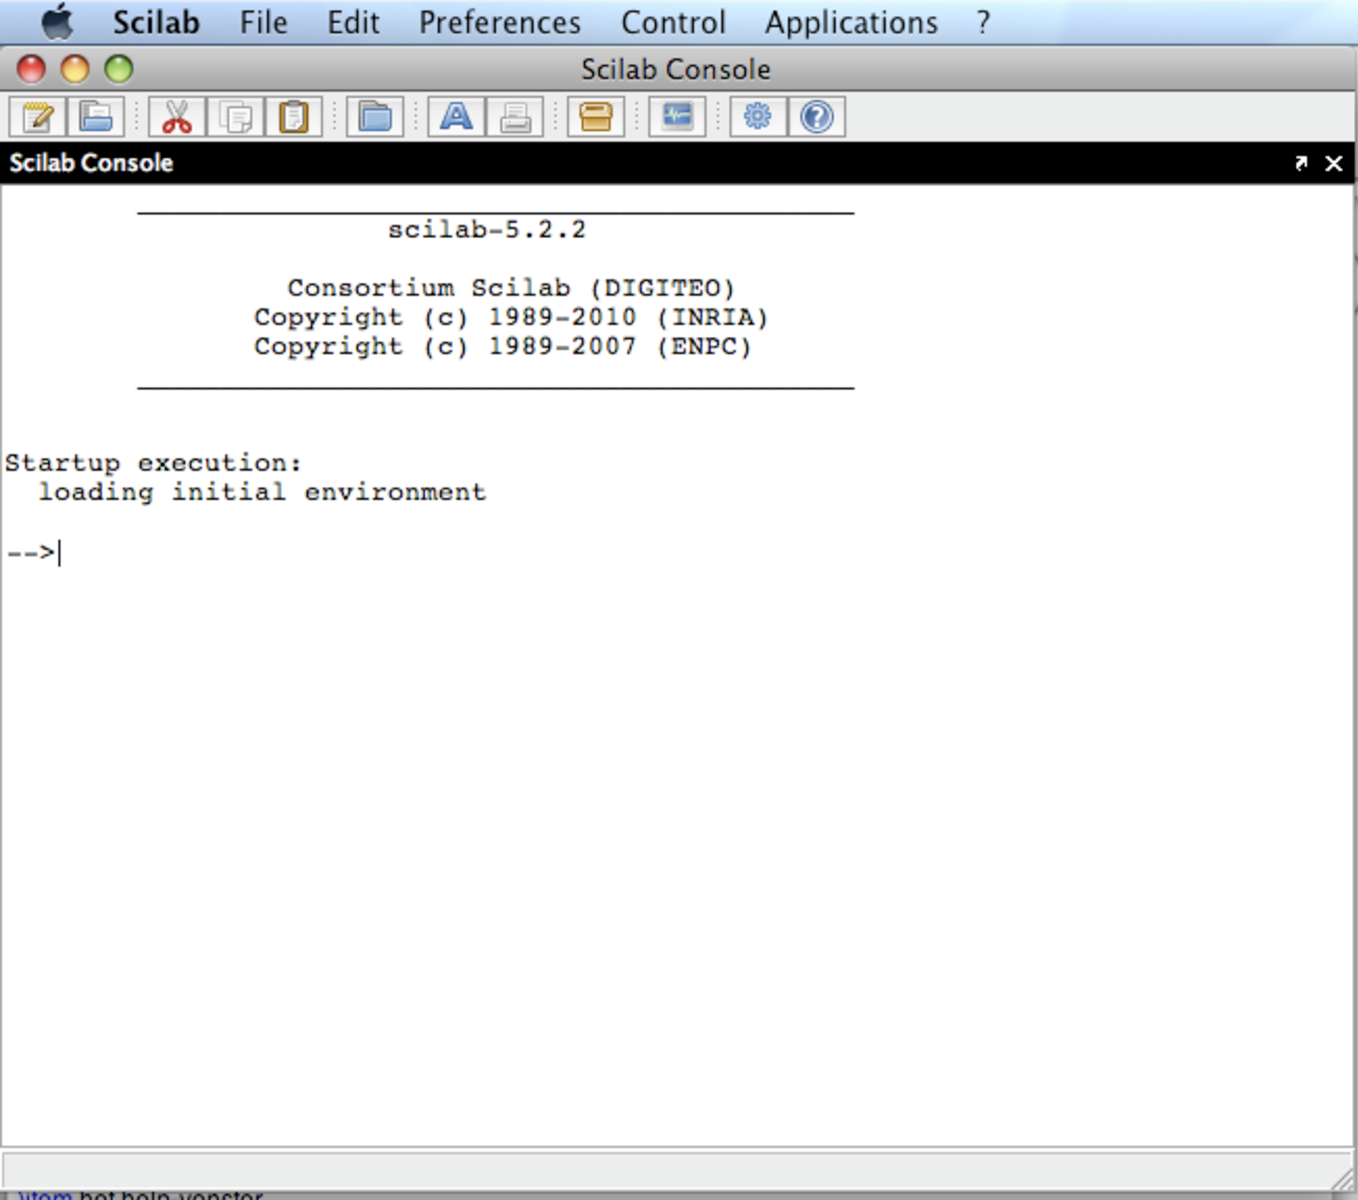
\includegraphics[width=\textwidth, trim= 0cm 10cm 0cm 0cm, clip]{figuren/scilab/01console}
  \caption{Console van Scilab}
	\label{fig:console}
	\end{center}
\end{figure}

Instructies worden ingevoerd na de prompt (\verb+-->+) via het toetsenbord en worden uitgevoerd door de return-toets in te drukken. Een vorige regel kan je laten uitvoeren door met de pijltjestoetsen te werken. Het console venster kan je leegmaken met de toets \verb+F2+.

\subsection{Rekenen met getallen}

Het programma kent de bewerkingen \verb0+0, \verb+-+, \verb+*+, \verb0/0 en voor de machtsverheffing \verb+^+. Als de exponent uit meerdere termen bestaat, dan plaatsen we die tussen haakjes.
Het decimaal punt wordt met een punt genoteerd (en geen komma).  Meerdere instructies worden van elkaar gescheiden d.m.v.\ een komma. Output wordt onderdrukt door gebruik te maken van de puntkomma ';'.


\begin{lstlisting}[caption={Eenvoudige bewerkingen}, label={eenvoudigebewerkingen}]
-->4+5.5
  ans =

     9.5

-->3*4^2-10,-1^2*3+7,(-1)^(2*3)+7
  ans =
	
     38.
  ans =

     4.
  ans =
     8.
-->sqrt(25)+6;
 
-->
\end{lstlisting}

Scilab is hoofdlettergevoelig. Bijvoorbeeld voor de vierkantswortel:


\begin{lstlisting}[caption={Vierkantswortel}, label={vierkantswortel}]
-->sqrt(25), sqrt(368)
 ans  =
 
    5.  
 ans  =
 
    19.183326
    
-->SQRT(9)
        !--error 4 
Undefined variable: SQRT     
\end{lstlisting}


Constanten zoals $\pi$, $e$, t (true) en f (false) worden voorafgegaan door \%.

\begin{lstlisting}[caption={Constanten}, label=constanten]
-->%pi,%e 
 %pi  =
 
    3.1415927  
 %e  =
 
    2.7182818  
 \end{lstlisting}


Scilab heeft een aantal ingebouwde functies zoals \verb+log()+, \verb+abs()+, \verb+ceil()+,\\ \verb+floor()+, \verb+modulo(n,m)+, \verb+sin()+, \verb+cos()+ \ldots\ Je kan de tab-toets gebruiken om de naam van een functie aan te vullen als je slechts de eerste letters van de functienaam weet (figuur \ref{fig:tabtoets}). Merk op dat --\,in tegenstelling tot de gangbare rekenmachines\,-- de functie \verb/log()/ de logaritmische functie is met grondtal \verb/e=2.7182818/ en niet met grondtal 10.

\begin{lstlisting}[caption={Enkele ingebouwde functies}, label=ingebouwdefuncties]
-->abs(-5),floor(6.3),log(30),modulo(25,3)
  ans =

     5.
   ans =

     6.
  ans =

     3.4011974
  ans =

     1.
\end{lstlisting}

\begin{figure}[h!t]
   \begin{center}
    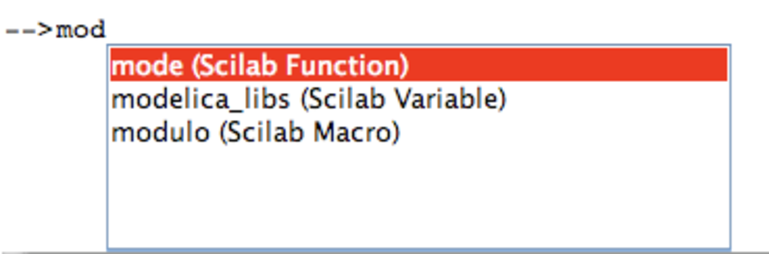
\includegraphics[width=0.8\textwidth]{figuren/scilab/02tabtoets}
  \caption{Gebruik de tabtoets als je een functienaam niet meer volledig weet.}
	\label{fig:tabtoets}
	\end{center}
\end{figure}

\newpage
\subsection{De editor}

Rechtstreeks werken in de console heeft een belangrijk aantal beperkingen: als je een bewerking over meerdere lijnen schrijft, kan je de vorige lijnen niet meer corrigeren. Vanaf versie 5.4 kan je weliswaar een sessie  opslaan(`save environment'), maar het is niet zo handig.  Het is daarom beter om de editor te gebruiken. Je opent het venster als je klikt op het eerste icoontje in de toolbar van de console of via de menubalk: Applications - SciNotes.

In de editor kan je meerdere bewerkingen op dezelfde lijn zetten. Je moet ze dan scheiden met een komma of puntkomma. Dit komt de leesbaarheid wel niet ten goede. Je kan de code documenteren door een lijn te beginnen met \verb+//+. 

\begin{figure}[h!t]
   \begin{center}
    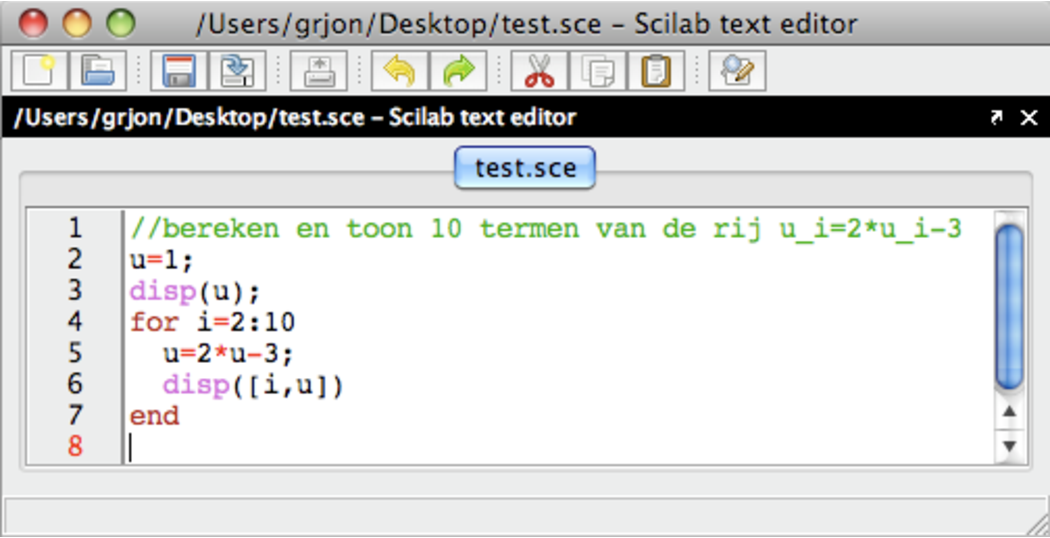
\includegraphics[width=\textwidth]{figuren/scilab/03editor}
  \caption{Schrijven in de editor}
	\label{fig:editor}
	\end{center}
\end{figure}

De code die je typt in de editor kan je opslaan in de editor als een bestand met extensie \verb+.sce+. Als het opgeslagen is, kan je het inladen en uitvoeren in de console via het menu-item Execute. Als je maar een gedeelte van het bestand wil laten uitvoeren, selecteer je het met de muis, klik je rechts en kies je `Evaluate Selection'.

Als je werkt met Mac OS X, moet je de line-endings veranderen naar het unix-formaat (Scilab- Preferences - SciNotes - Default end of line - Unix (LF)). Indien je dit niet doet, wordt slechts de eerste regel van het bestand uitgevoerd.

\subsection{Het grafisch venster}
Telkens je een functie of grafiek laat tekenen (zie sectie~\ref{sec:grafiek}) opent het grafisch venster. Een voorbeeld krijg je als je \verb+plot+ typt in de console.  Met het commando \verb/clf/ (\emph{clear figure}) wordt het grafisch venster opgeschoond. 

Het is mogelijk om verschillende grafische vensters tegelijk te openen (figuur ~\ref{fig:grafisch_venster}). Je opent een nieuw venster met het commando \verb+scf(n)+. Met datzelfde commando kan je van het ene naar het andere venster gaan om bijvoorbeeld een  nieuwe figuur te tekenen in het eerste venster. 
\begin{figure}[h!t]
   \begin{center}
    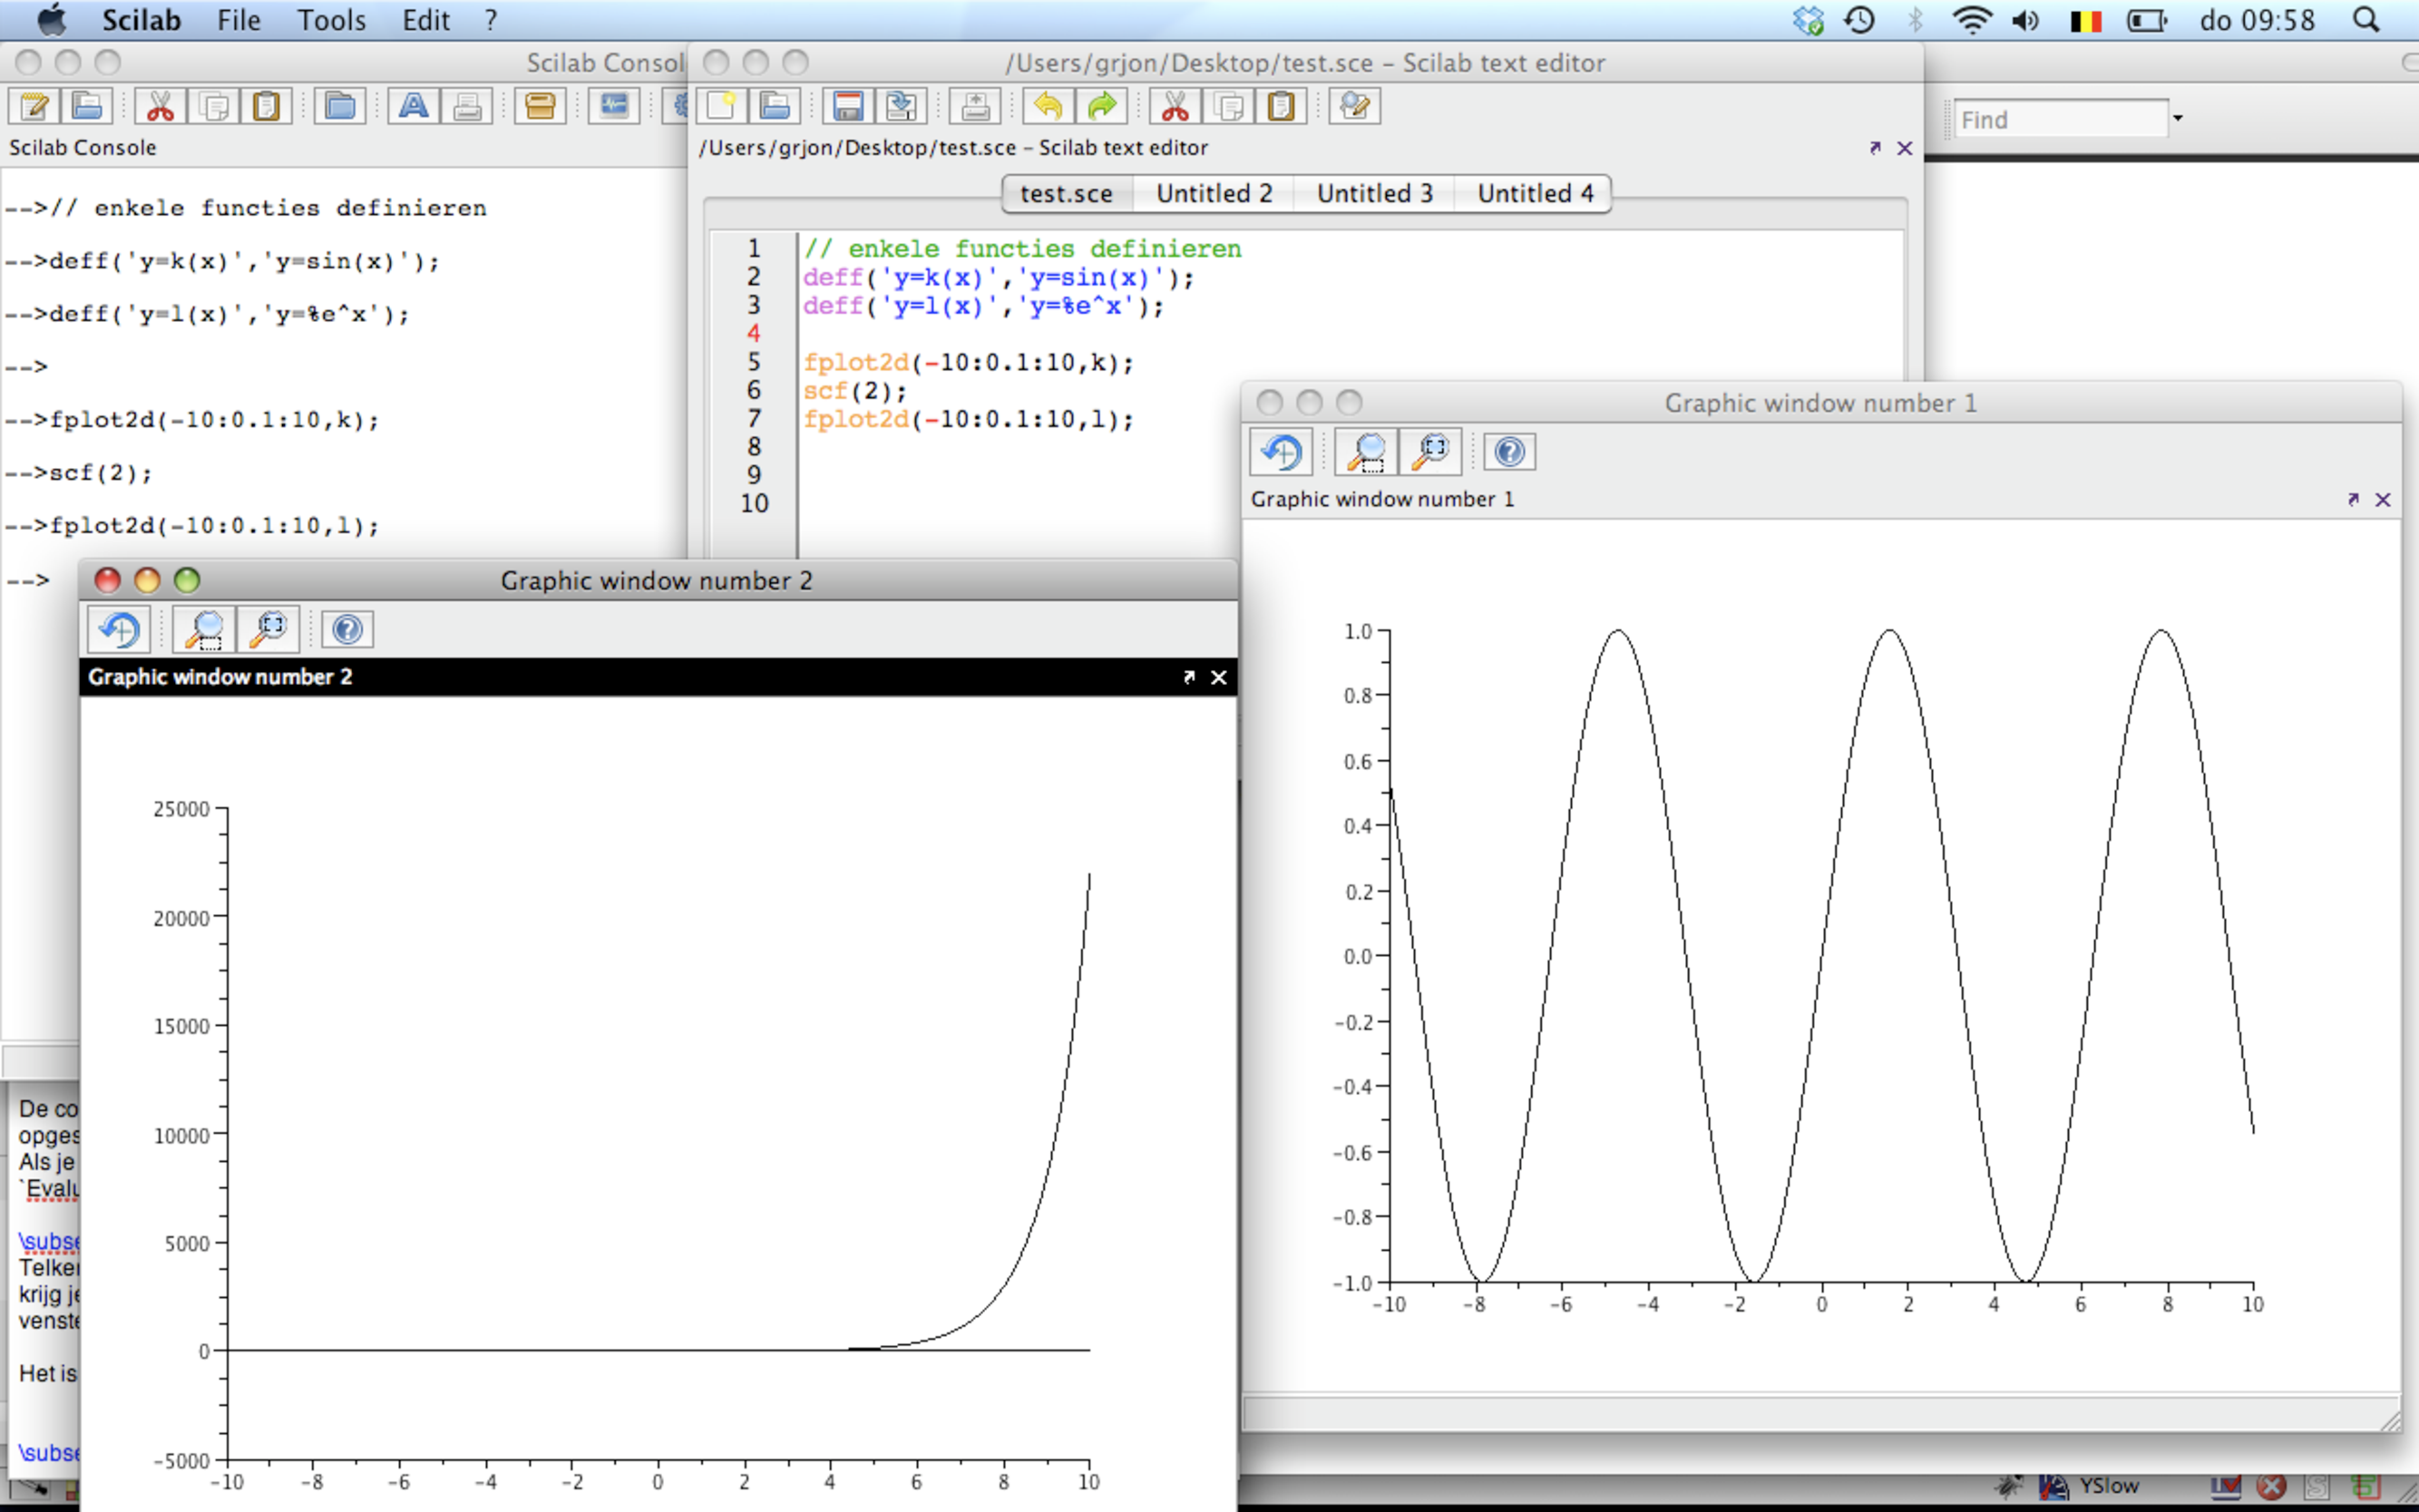
\includegraphics[width=\textwidth]{figuren/scilab/04grafisch_venster}
  \caption{Meerdere grafieken tonen}
	\label{fig:grafisch_venster}
	\end{center}
\end{figure}

\subsection{Het help venster}
Scilab beschikt over een uitgebreide helpfunctie. Als je op het vraagteken klikt of \verb+help+ typt in de console, opent een helpvenster met zoekfunctie (figuur \ref{fig:helpvenster}). Je kan ook specifieke informatie vragen over een functie door bijvoorbeeld in de console \verb+help functienaam+ in te typen. Tenslotte kan je in SciNotes een functie selecteren, rechts klikken en kiezen voor `help on selection' (zie figuur~\ref{fig:helpOnSelection}). Het help-venster opent zich en toont de info over de geselecteerde functie.

\begin{figure}[h!t]
   \begin{center}
    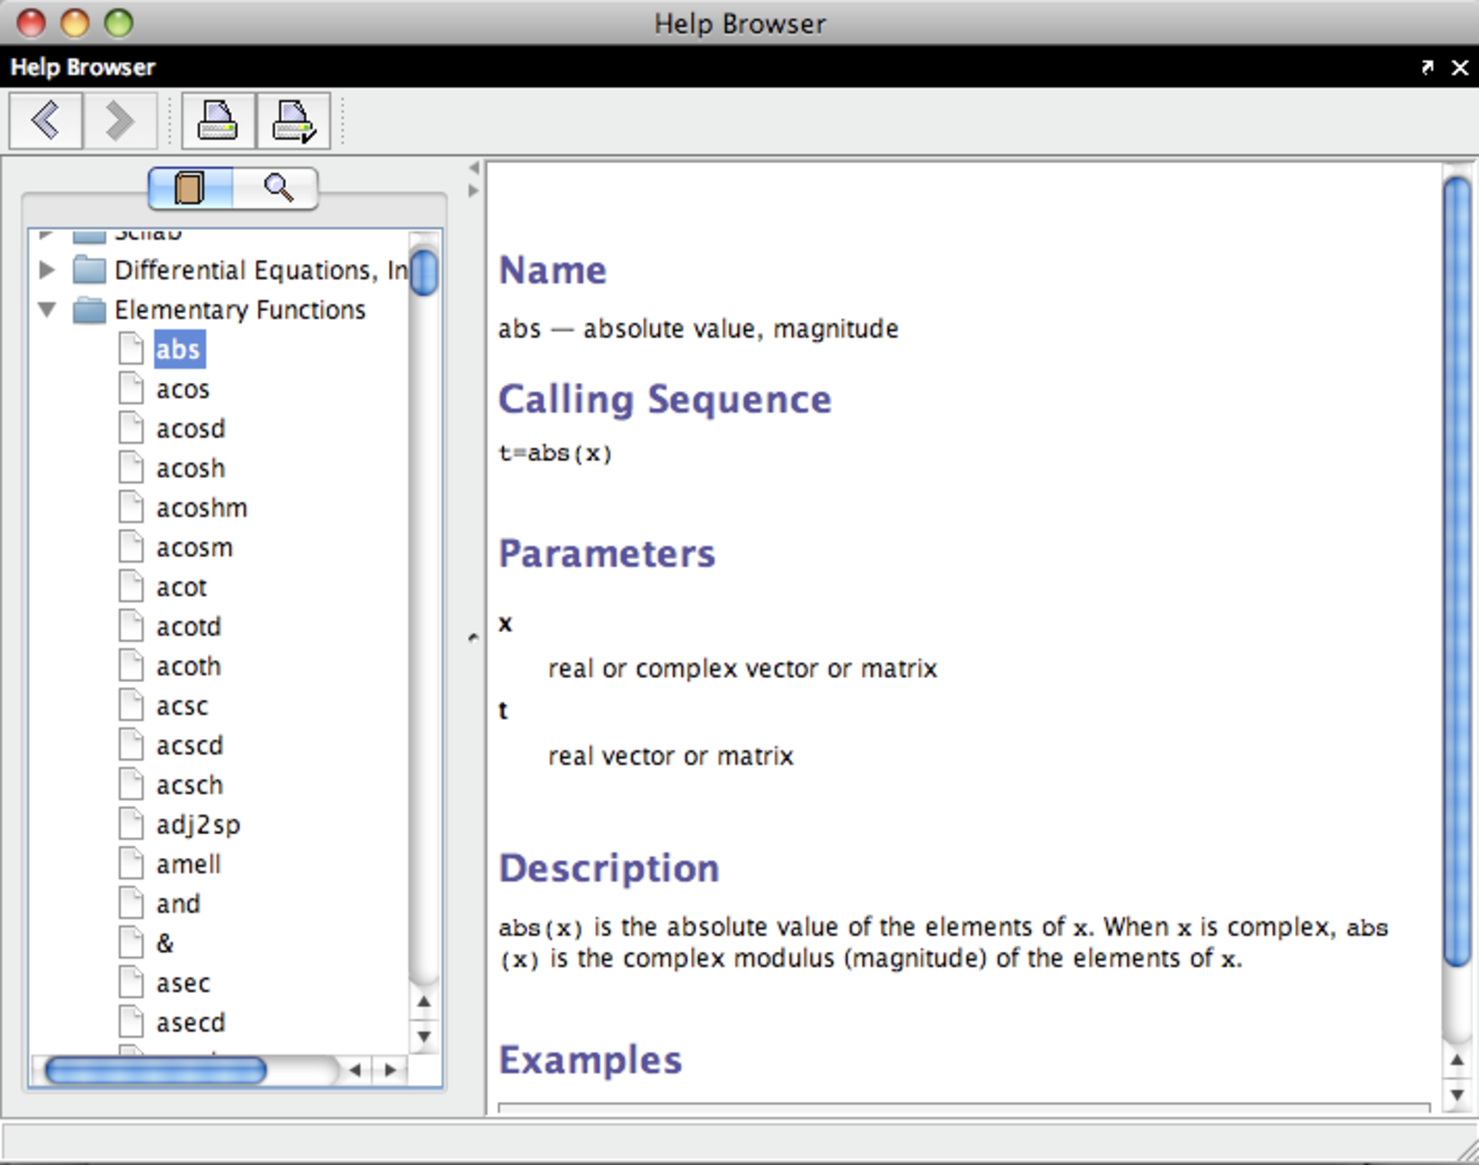
\includegraphics[width=\textwidth]{figuren/scilab/05helpvenster}
  \caption{Het helpvenster}
	\label{fig:helpvenster}
	\end{center}
\end{figure}

\begin{figure}[htbp]
\centering
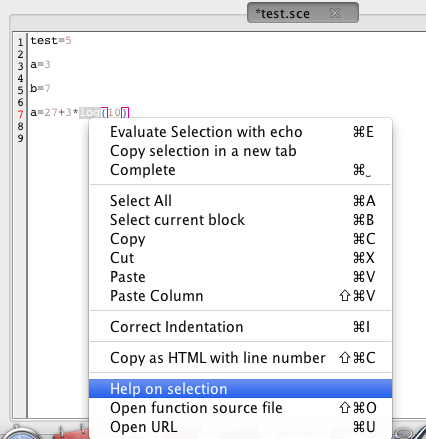
\includegraphics[width=0.7\textwidth]{figuren/scilab/05bhelp_in_scinotes}
\caption{`Help on selection' in SciNotes}
\label{fig:helpOnSelection}
\end{figure}

\subsection{Het scherm met veranderlijken}
Het scherm met veranderlijken (`variable window', figuur~\ref{fig:05cvariableWindow}) toont alle veranderlijken die je tot nog toe gedefinieerd hebt. Als je dubbelklikt op een naam, kan je de waarde aflezen. 
\begin{figure}[htbp]
\centering
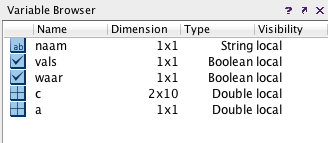
\includegraphics[width=0.7\textwidth]{figuren/scilab/05cvariableWindow}
\caption{Het scherm met veranderlijken}
\label{fig:05cvariableWindow}
\end{figure}

\subsection{Commando overzicht}
Het commando overzicht toont een chronologisch overzicht van de commando's die je tijdens de huidige sessie uitvoerde (`command history'). Als je op een commando dubbelklikt, wordt het opnieuw uitgevoerd. Je kan rechts klikken op een commando en dan kiezen dat je kopieert naar SciNotes.

\subsection{Verschillende vensters combineren}

Doordat je met verschillende vensters tegelijk werkt (console, editor, grafisch venster etc) wordt je scherm al snel een warboel. Je kan de verschillende kleine vensters ook combineren tot één groot venster (figuur~\ref{fig:verschillendevensters}). Neem een venster vast met de muis bij de \emph{blauwe} balk bovenaan en sleep het naar de gewenste positie in een ander venster. Als je het bronvenster laat samenvallen met het doelvenster, worden beide vensters over mekaar geplaatst en kan je van het ene venster naar het andere gaan door middel van de tabs. Als je verschillende vensters van de editor opent, verschijnen ook de tabs (zie figuur~\ref{fig:06bverschillendevensters}). 

\begin{figure}[h!t]
   \begin{center}
    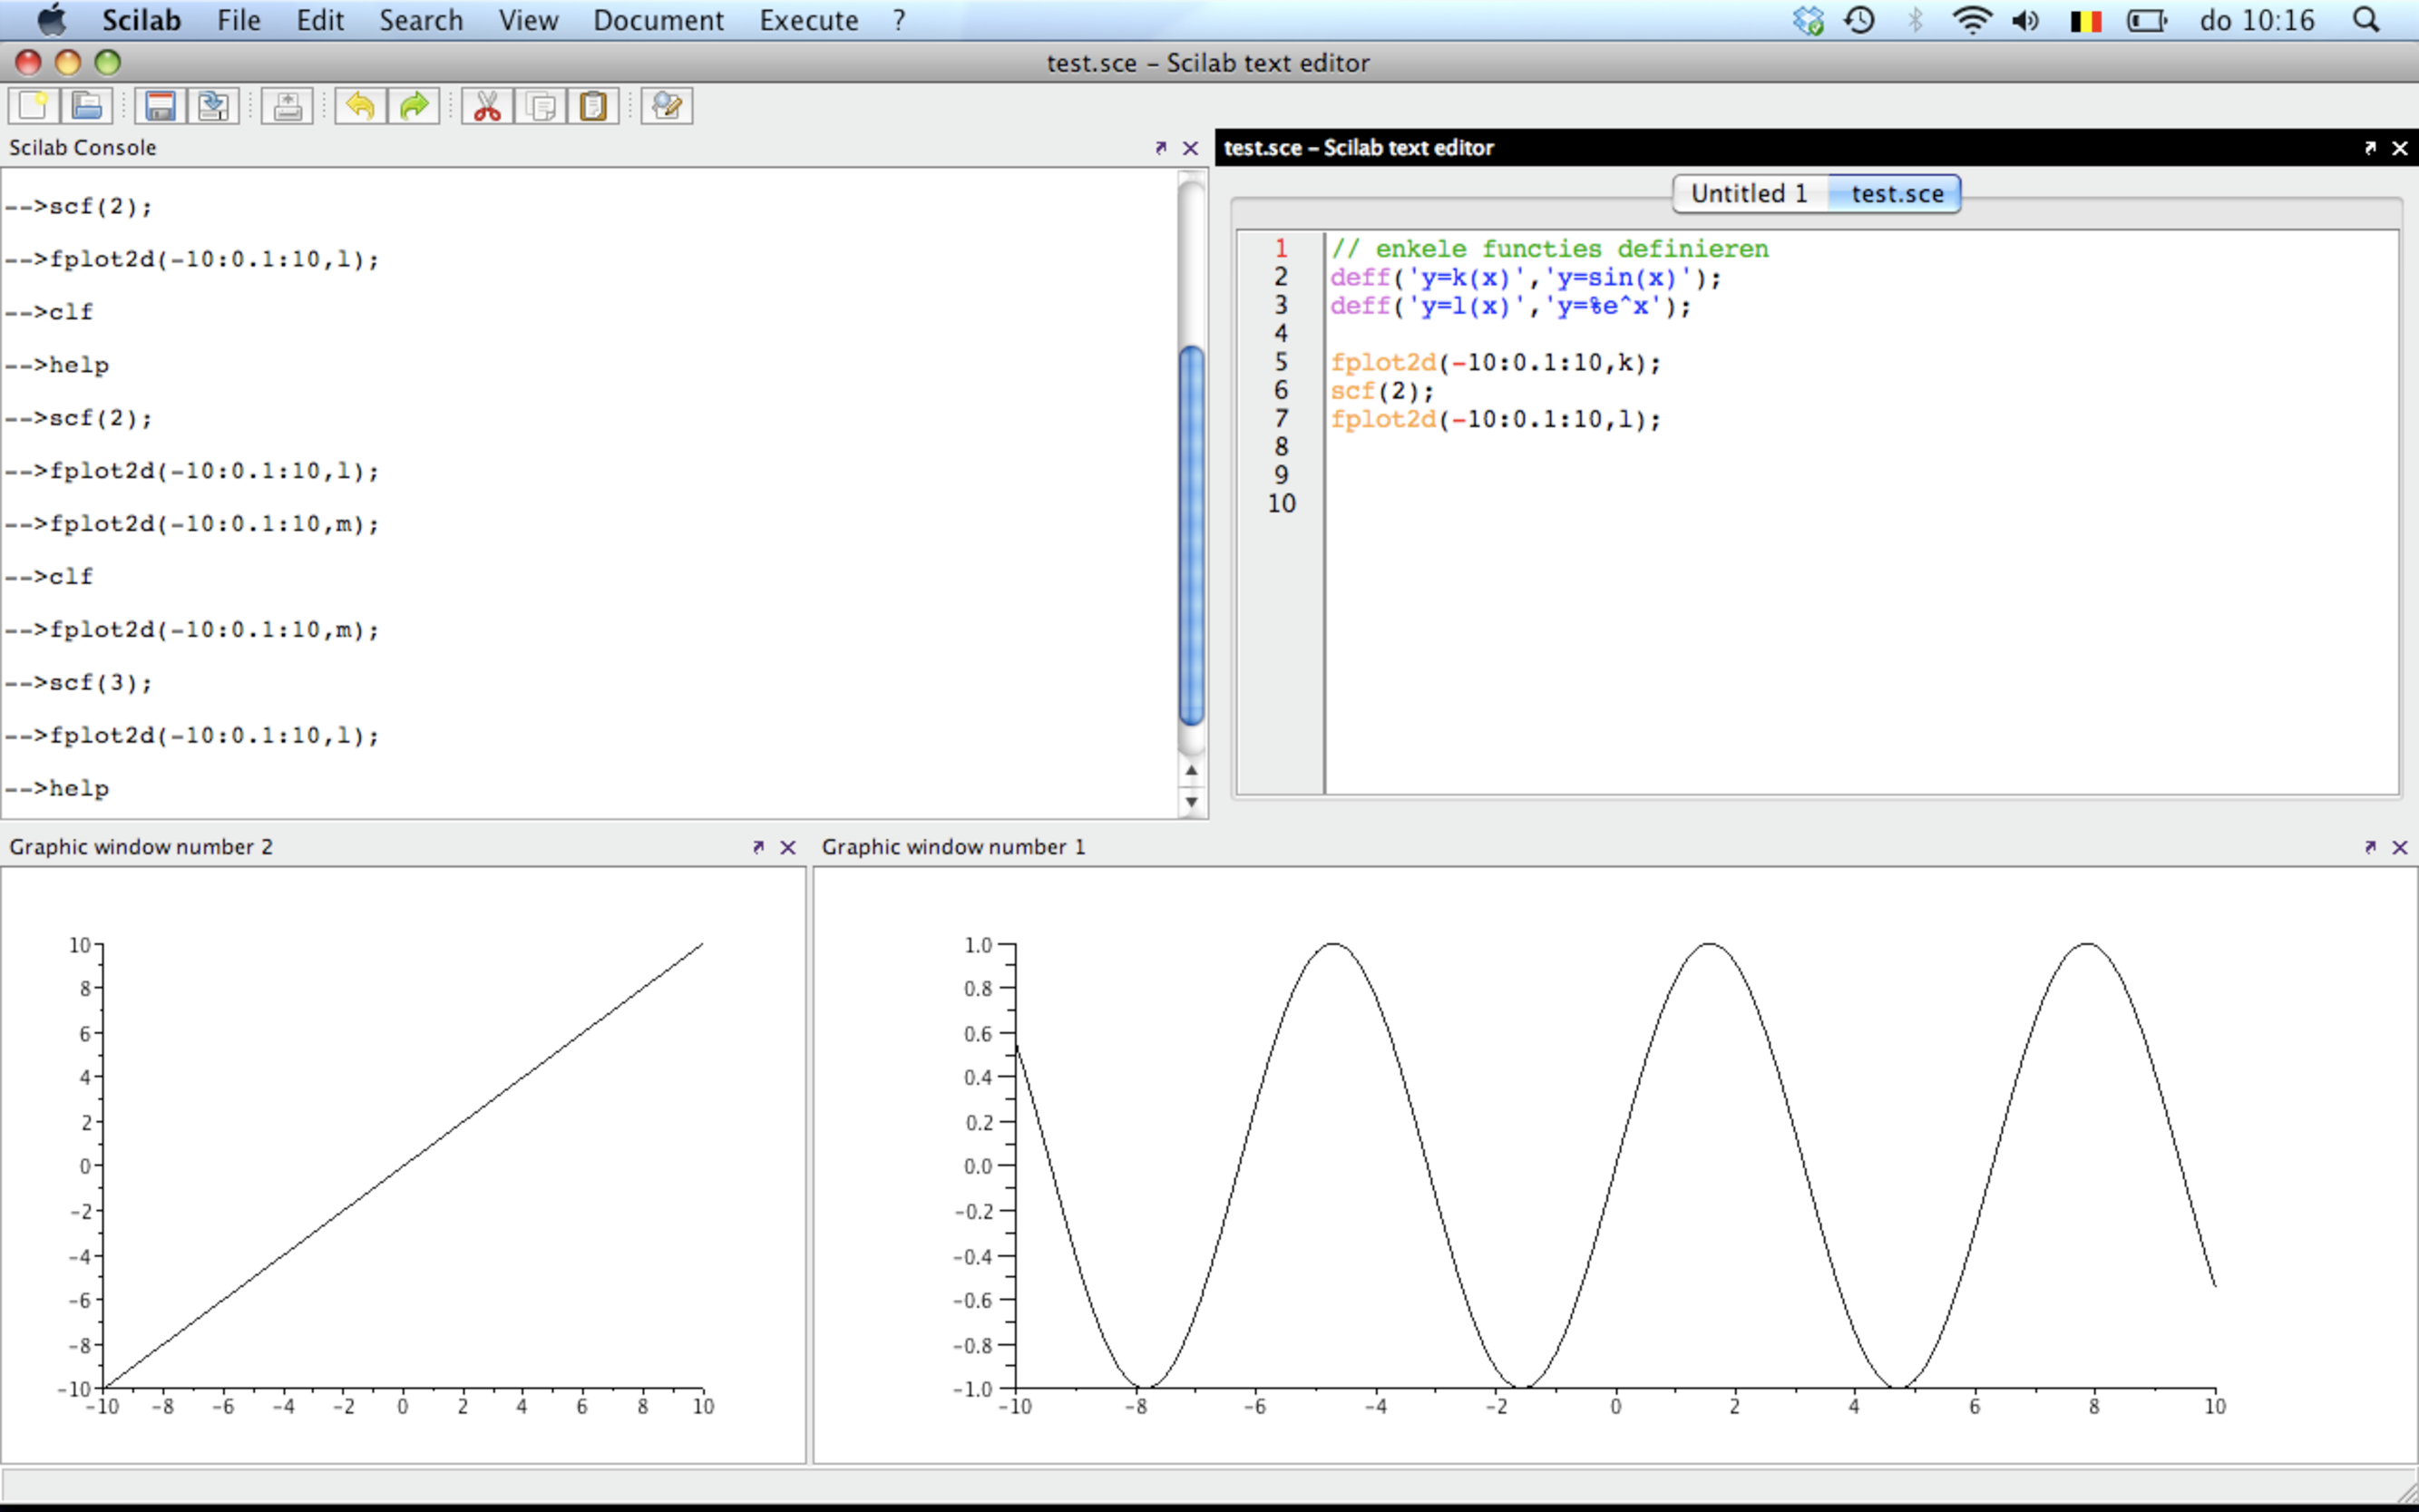
\includegraphics[width=\textwidth]{figuren/scilab/06verschillendevensters.pdf}
  \caption{Verschillende vensters gecombineerd in één venster}
	\label{fig:verschillendevensters}
	\end{center}
\end{figure}

\begin{figure}[htbp]
\centering
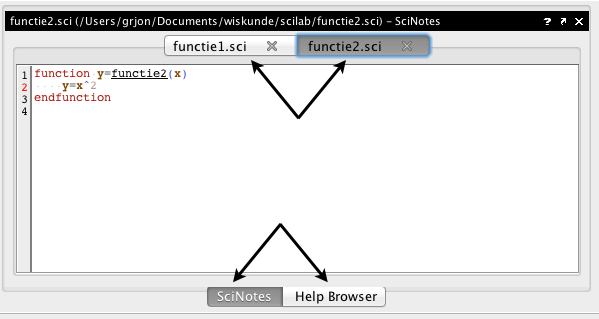
\includegraphics[width=\textwidth]{figuren/scilab/06bverschillendevensters}
\caption{Er verschijnen tabs als je verschillende vensters over mekaar plakt}
\label{fig:06bverschillendevensters}
\end{figure}

%\clearpage
\section{Werken met variabelen}
Variabelen hoeven in Scilab niet eerst gedeclareerd te worden. Een variabele is wel pas gekend als er een waarde aan toegekend is.

\begin{lstlisting}[caption={Foutmelding bij niet-gedefinieerde variabele}, label=Foutmelding bij niet-gedefinieerde variabele]
-->a
  !--error 4 
Undefined variable: a
\end{lstlisting}

Als er een waarde toegekend wordt aan \verb+a+ is er geen foutmelding meer.
\begin{lstlisting}[caption={De waarde van een variabele}, label=De waarde van een variabele]
-->a=%pi/4;
 
-->a
 a  =
 
    0.7853982  
\end{lstlisting}

De naam van een variabele kan bestaan uit meerdere karakters. Een waarde toekennen aan de variabele gebeurt d.m.v.\ `='. Als deze variabele nadien gebruikt wordt in wiskundige uitdrukkingen, dan wordt er gewerkt met de waarde van de variabele. 

\begin{lstlisting}[caption={Waarde van variabelen}, label=waardevanvariabelen]
-->x=-2,3*x^3-1
  x =
     
     -2.
  ans =
     
     -25.
\end{lstlisting}

Als er geen naam toegekend wordt aan een berekening, wordt de waarde automatisch toegekend aan de veranderlijke \verb+ans+.
\begin{lstlisting}[caption={De variabele ans}, label=ans]
-->257/3
 ans  =
 
    85.666667  
 
-->y=ans*3
 y  =
 
    257.  
\end{lstlisting}

Scilab kent verschillende datatypes. De belangrijkste in het kader van dit OPO zijn real, boolean, integer, string en matrices. Er zijn verschillende functies beschikbaar om het datatype van een veranderlijke te testen (bijvoorbeeld isnum, isletter). We merken op dat intern in het systeem alle veranderlijken opgeslagen worden als matrix (zie sectie~\ref{sec:scilabMatrices}). 

Als je het zou willen, zou je aan dezelfde variabele  achtereenvolgens een ander datatype kunnen toekennen. Dit wordt geïllustreerd in listing~\ref{datatype}.

\begin{lstlisting}[caption={Verschillend datatype toekennen aan dezelfde veranderlijke}, label=datatype]
-->x=1
 x  =
    1.  
-->x+1
 ans  =
    2.  
-->x='voor'
 x  =
 voor   
-->x+'deur'
 ans  =
 voordeur  
 \end{lstlisting}



\section{Vectoren en matrices}
\label{sec:scilabMatrices}
Een vector is een geordende verzameling van getallen. In programmeervakken noem je dit meestal een \emph{eendimensionale array}. Een voorbeeld:
\begin{displaymath}
V=[1,2,3,4,5]
\end{displaymath}
Een matrix is een rechthoekig schema getallen (\emph{tweedimensionale array}). 
\begin{displaymath}
M=\begin{bmatrix}
 1&2  &-3 &2 \\
 8& 5 &7 &5 \\
 -6& -4 &11&8
\end{bmatrix}\,.
\end{displaymath}

Bovenstaande matrix bijvoorbeeld bevat 3 rijen en 4 kolommen. In Scilab wordt een matrix  rij per rij genoteerd tussen vierkante haken `\verb+[,]+'. De kolommen worden gescheiden door `\verb+,+' en de rijen door `\verb+;+'. Het aantal rijen en kolommen wordt opgevraagd door de functie \verb+size()+. Merk op dat deze functie als antwoord een vector met twee elementen geeft.

\begin{lstlisting}[caption={Een matrix defini\"eren}, label=Matrixdef]
-->M=[1,2,-3,2;8,5,7,5;-6,-4,11,8]
 M  =
 
    1.    2.  - 3.     2.  
    8.    5.    7.     5.  
  - 6.  - 4.    11.    8.  
  
  -->size(M)
 ans  =
 
    3.    4.  
\end{lstlisting}

Als de vector bestaat uit een \emph{rij opeenvolgende getallen of een rekenkundige rij}, volstaat het om de korte notatie met `\verb+:+' te gebruiken (zie listing~\ref{korte_notatie}). Als het verschil gelijk is aan 1, hoeft het niet expliciet vermeld te worden (eerste voorbeeld). Als het verschil een ander getal is, moet het expliciet vermeld worden (tweede voorbeeld). Vierkante haken mogen, maar zijn niet nodig.
\begin{lstlisting}[caption={Een matrix defini\"eren: korte notatie}, label=korte_notatie]
-->B=[1:8]
 B  =
 
    1.    2.    3.    4.    5.    6.    7.    8.  
 
-->C=3:-0.5:0
 C  =
 
    3.    2.5    2.    1.5    1.    0.5    0.  
 
\end{lstlisting}


Een matrixelement wordt opgevraagd door de indices te geven, bvb.: \verb+M(1,2)+ (let op: hier ronde haakjes gebruiken). Dit is het element in de eerste rij, tweede kolom. In bovenstaand geval zou dit \verb+2+ opleveren. In tegenstelling tot programmeertalen als Java en PHP heeft het eerste element uit een rij index 1 en niet index 0. 
Een vector is niets meer dan een matrix bestaande uit 1 rij of 1 kolom. Om een element uit een vector te halen moet je slechts \'e\'en index meegeven.

Scilab kent heel wat ingebouwde functies voor matrices en vectoren. In tabel~\ref{tabel:matrices} sommen we er enkele op.

\begin{table}[h] \small
\centering
\caption{Enkele ingebouwde functies m.b.t.\ matrices}
\begin{tabular}{p{7.cm}p{4.cm}}
\toprule

definitie matrix    &   \verb+M=[1,2,3,4;5,6,7,8]+ \\

matrixelement       &   \verb+M(2,3)+\\

volledige rij van een matrix    & \verb+M(3,:)+\\

submatrix           & \verb+M(1:2,2:3)+\\

matrices samenvoegen: onder mekaar            & \verb+M=[A;B]+\\
matrices samenvoegen: langs mekaar            &\verb+M=[A,B]+\\
matrix transponeren (rijen$\leftrightarrow$kolommen) & M'\\

constante optellen bij elk element & \verb/M+3/ \\

elk element vermenigvuldigen met constante & \verb+M*3+ \\

matrixoptelling: element per element	& \verb/M+N/\\

matrixvermenigvuldiging 	& \verb/M*N/\\
$\qquad$(let op de dimensies!)&\\

matrixvermenigvuldiging: 	& \verb/M.*N/\\
$\qquad$element per element&\\

macht van een matrix	& \verb/M^2/\\
$\qquad$element per element&\\

matrix met $4$ rijen en $2$ kolommen,               & \verb+zeros(4,2)+ \\
$\qquad$ieder element gelijk aan $0$ &\\

idem, maar ieder element gelijk aan $1$ & \verb+ones(4,2)+ \\

idem, ieder element random tussen 0 en 1 & \verb+rand(4,2)+ \\
lengte van de vector $V$ & \texttt{length(V)} \\
aantal rijen en kolommen van de matrix $A$ & \texttt{size(A)} \\
elementen van $A$ sorteren&\texttt{gsort(A)}\\
elementen van $A$ kleiner dan 5, gelijk aan 3& \verb+find(A<5)+, \verb+find(A==3)+\\
\bottomrule
\end{tabular}
\label{tabel:matrices}
\end{table}

Zoek in de help van Scilab welke opties de functies \verb/gsort/ en \verb/find/ bieden. 


\section{Functies}

\subsection{Definitie van een functie}
\label{sec:werken_met_functies}
De definitie van een functie begint met \verb+function+ en eindigt met \verb+endfunction+. In listing~\ref{Functiedef} definiëren we de functie \verb+dollars+ die het bedrag \verb+e+ in euros omzet naar het bedrag \verb+d+ in dollars. De variabele \verb/t/ is de koerswissel, \verb/e/ en \verb+t+ zijn de \emph{variabelen}; \verb/d/ is het \emph{resultaat} (de return-waarde).
\begin{lstlisting}[caption={Functie defini\"eren}, label=Functiedef]
-->function d=dollars(e,t);
-->  d=e*t;
-->endfunction
 
-->dollars(200,1.2)
 ans  =
 
    240.  
\end{lstlisting}

Listing~\ref{Functiedef} toont een functiedefinitie in het consolevenster. \emph{Dat is niet de beste manier van werken}, maar het kan wel
voor functies die maar uit een paar regels tekst bestaan.

Voor een eenvoudige functie kan je ook  het commando \verb+deff+ gebruiken om een functie te defini\"eren in de commandolijn:
\begin{lstlisting}[caption={Functie defini\"eren met deff}, label=functiedeff]
-->deff('y=g(x)','y=x^2-1')

-->g(3)
 ans  =
 
    8.   
\end{lstlisting}

In de eerste string geef je mee dat je de functie \verb+g+ definieert die \verb+x+ als parameter heeft. In de tweede string (\verb+'y=x^2-1'+) zeg je hoe deze functie gedefinieerd is.

\subsection{Interactie met de gebruiker}

Soms verwacht een functie input van de gebruiker. Hiervoor kan je de functie \verb+input()+ gebruiken. Met dit commando wacht het programma op een waarde die via het toetsenbord wordt ingegeven. 

Met de functie \verb+disp+ kan je verzorgde output leveren. De functie \verb+string()+ verandert het datatype naar een string. Met het \verb/+/-teken plak je verschillende strings aan mekaar. Je kan ook de functie \verb/printf()/ gebruiken. Dit wordt geïllustreerd in figuur~\ref{fig:input}. Om output naar een bestand te schrijven gebruik je de functie \verb+fprintf()+. Zie de helpfunctie voor meer informatie.

\begin{figure}[h!t]
   \begin{center}
    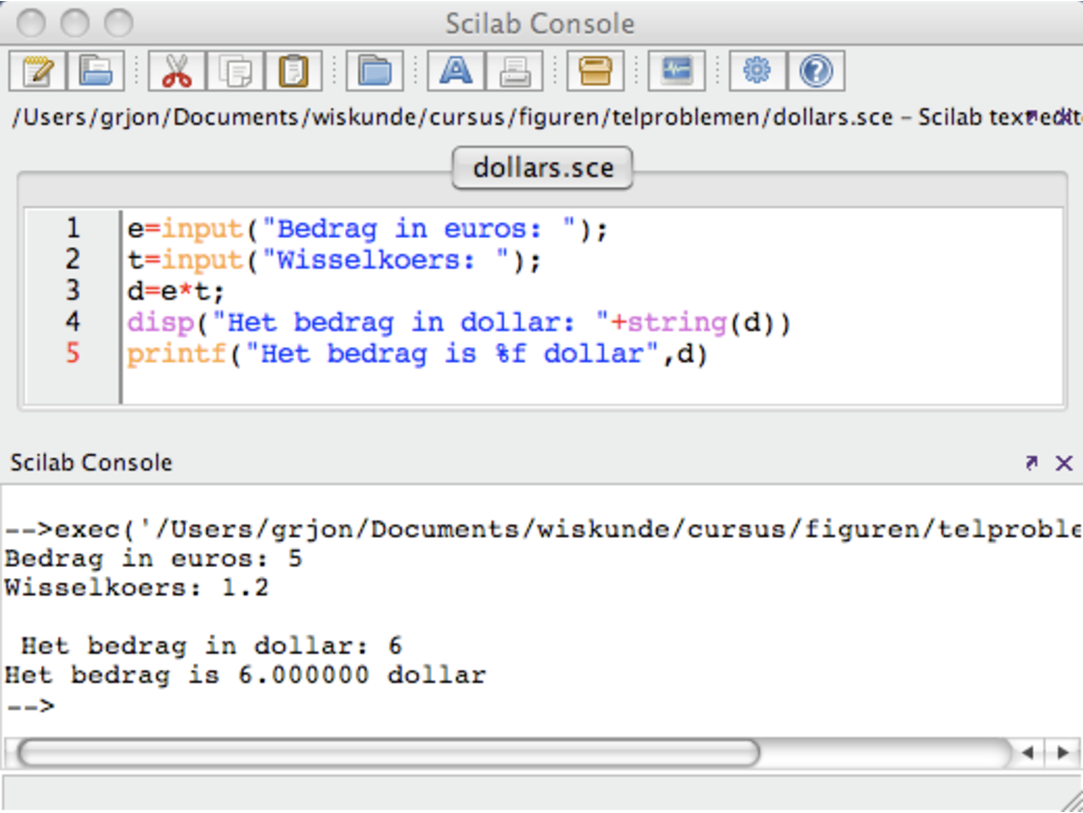
\includegraphics[width=\textwidth]{figuren/scilab/07input.pdf}
  \caption{Interactie met de gebruiker}
	\label{fig:input}
	\end{center}
\end{figure}

\subsection{Grafieken}
\label{sec:grafiek}
De grafiek van een functie is --\,naast de tabel en het functievoorschrift\,-- een handig middel om het verloop (nulpunten, stijgend en dalend, \dots) van de functie te beschrijven. De grafiek geeft een globaal beeld van de functie op een bepaald interval.

De ingebouwde functie \verb+plot(vec,function)+ genereert eenvoudig grafieken van functies. De veranderlijke \verb+vec+ is een vector. Voor alle elementen van deze vector wordt de functiewaarde berekend en in het grafisch venster geplot (zie figuur~\ref{figg:functie1}):

\begin{lstlisting}[caption={Functiedefinitie en plot}, label={Functiedefinitieenplot1}]	
function y=f(x)
  y=(x^2+2*x)*exp(-x)
endfunction
x=-2:0.2:5;
plot(x,f)
\end{lstlisting}

\begin{figure}[h!t]
   \begin{center}
  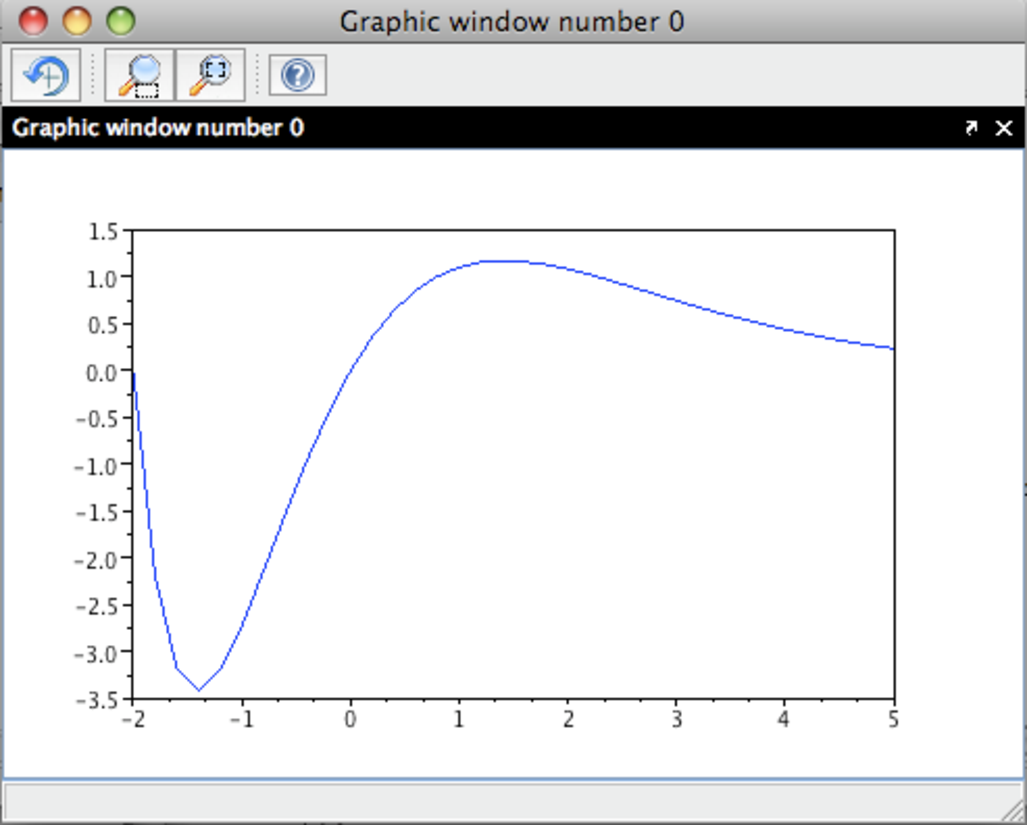
\includegraphics[width=0.8\textwidth]{figuren/scilab/08grafiek.pdf}
  \caption{Grafieken tekenen: resultaat van listing~\ref{Functiedefinitieenplot1}}
	\label{figg:functie1}
	\end{center}
\end{figure}


Merk op dat, als je twee maal achter mekaar \verb+plot+ invoert, beide grafieken over mekaar getekend worden.
Het commando \verb+clf+ (clear figure) zorgt ervoor dat het grafisch venster `opgeschoond' wordt. 

Tenslotte kan je je grafiek opfleuren met een titel, gridlijnen en kleurtjes (zie figuur~\ref{figg:meerderf}). In Windows kan je eenvoudig de eigenschappen van de grafieken wijzigen met het menu-item edit - figure properties (zie figuur~\ref{fig:11bgrafiek}). 
\begin{figure}[htbp]
\centering
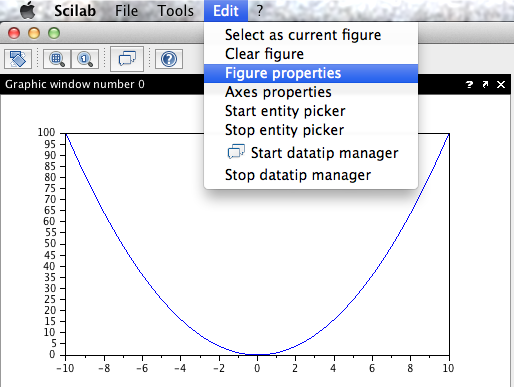
\includegraphics[width=\textwidth]{figuren/scilab/11bgrafiek}
\caption{De eigenschap van een grafiek veranderen met het venster voor eigenschappen}
\label{fig:11bgrafiek}
\end{figure}

Als je de eigenschappen van de grafiek niet via het menu kan wijzigen, kan je dat doen met behulp van de functie \verb+gda()+. Deze functie creëert een object met alle eigenschappen van de grafiek zoals kleuren, achtergrondvulling, al dan niet een titel etc. Voer het commando uit in de prompt om zijn waarde te kennen (zonder puntkomma!) en test zelf een aantal mogelijkheden uit.


\begin{lstlisting}[caption={Meerdere functies in \'e\'en grafiek}, label=meerderefunctiesplotten]	
function y=f(x)
  y=(x^2+2*x)*exp(-x)
endfunction
function y=g(x)
  y=sin(x/2)
endfunction
x=-2:0.1:5;
clf;
a=gda(); 
a.x_location="middle";
a.y_location="middle";
xtitle("De functies f(x) en g(x)");
xgrid(0); //het cijfer geeft de kleur aan
plot(x,f);
plot(x,g,'r');
\end{lstlisting}

\begin{figure}[h!t]
   \begin{center}
    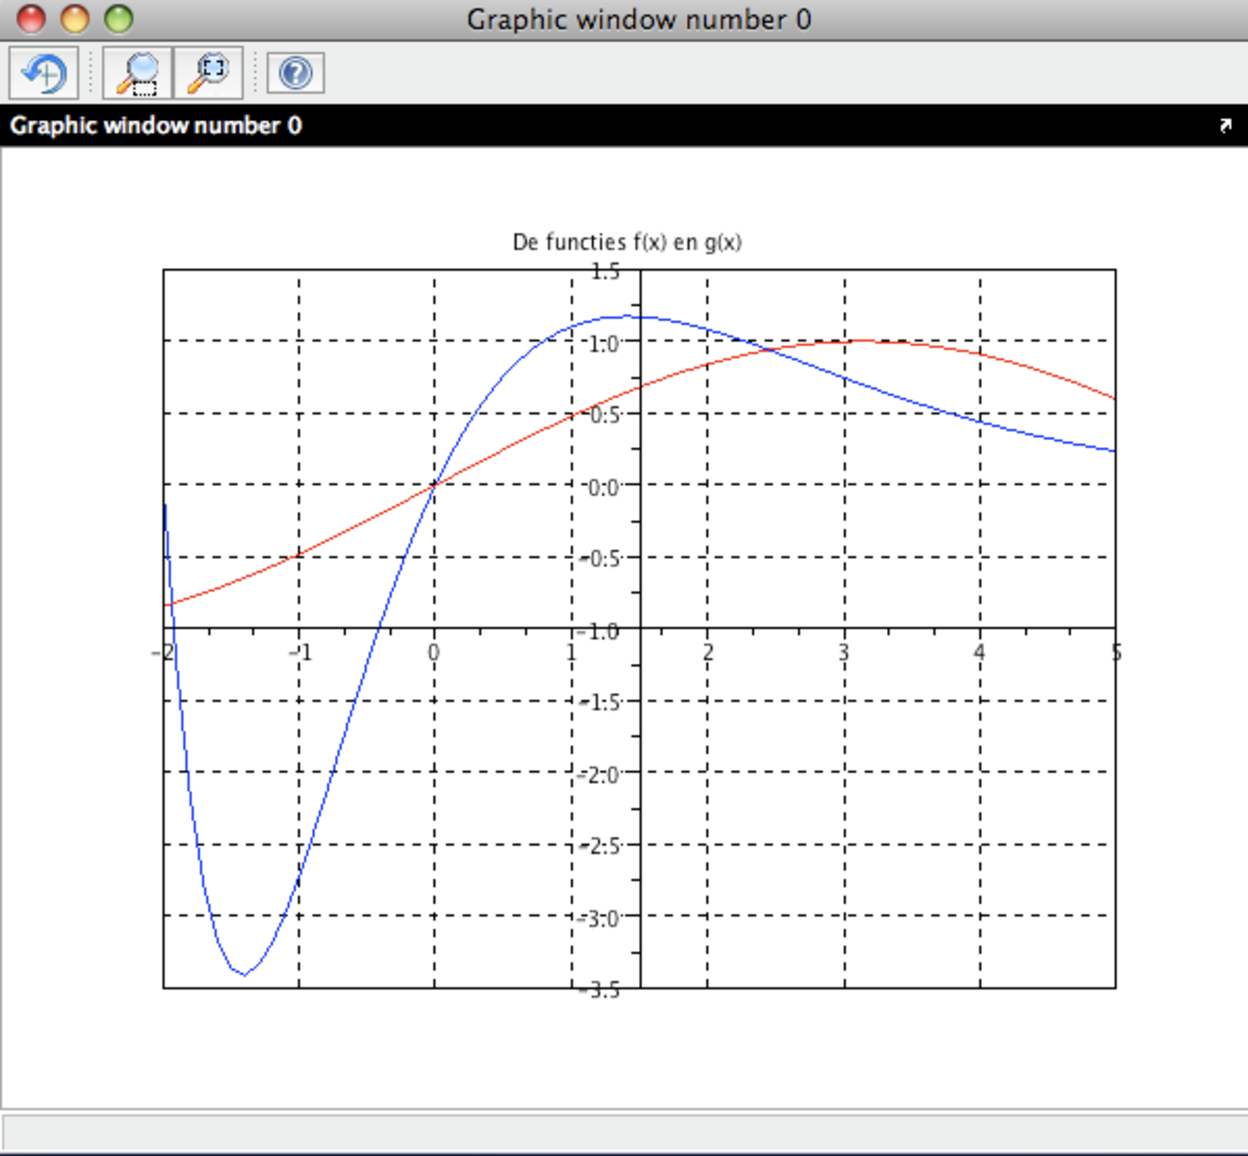
\includegraphics[width=0.8\textwidth]{figuren/scilab/10grafiek.pdf}
  \caption{Grafieken tekenen: resultaat van listing~\ref{meerderefunctiesplotten}}
	\label{figg:meerderf}
	\end{center}
\end{figure}


 
Nog een voorbeeld vind je in figuur \ref{figg:vierkant} (vooral te gebruiken in 2Ti). We maken hier gebruik van de functie \verb+plot2d+ om meer opties te bekomen.
\begin{lstlisting}[caption={Vierkant tekenen}, label=plot2d]	
clf;
a=gda(); 
a.x_location="bottom";
a.y_location="left";
// er moet rekening gehouden worden met de data_bounds
a.tight_limits="on";
// definieer de x- en y-range van de assen
a.data_bounds=[0,5,0,5];
// Definieer een titel en zorg ervoor dat hij getoond wordt
a.title.text="Een rechthoek";
// toon gridlijnen
xgrid(0);
a.thickness=1;
a.font_size=0.5;
x=[2,2,4,4,2]; y=[0,2,2,0,0];
plot2d(x,y)    
 \end{lstlisting}
 
\begin{figure}[h!t]
   \begin{center}
    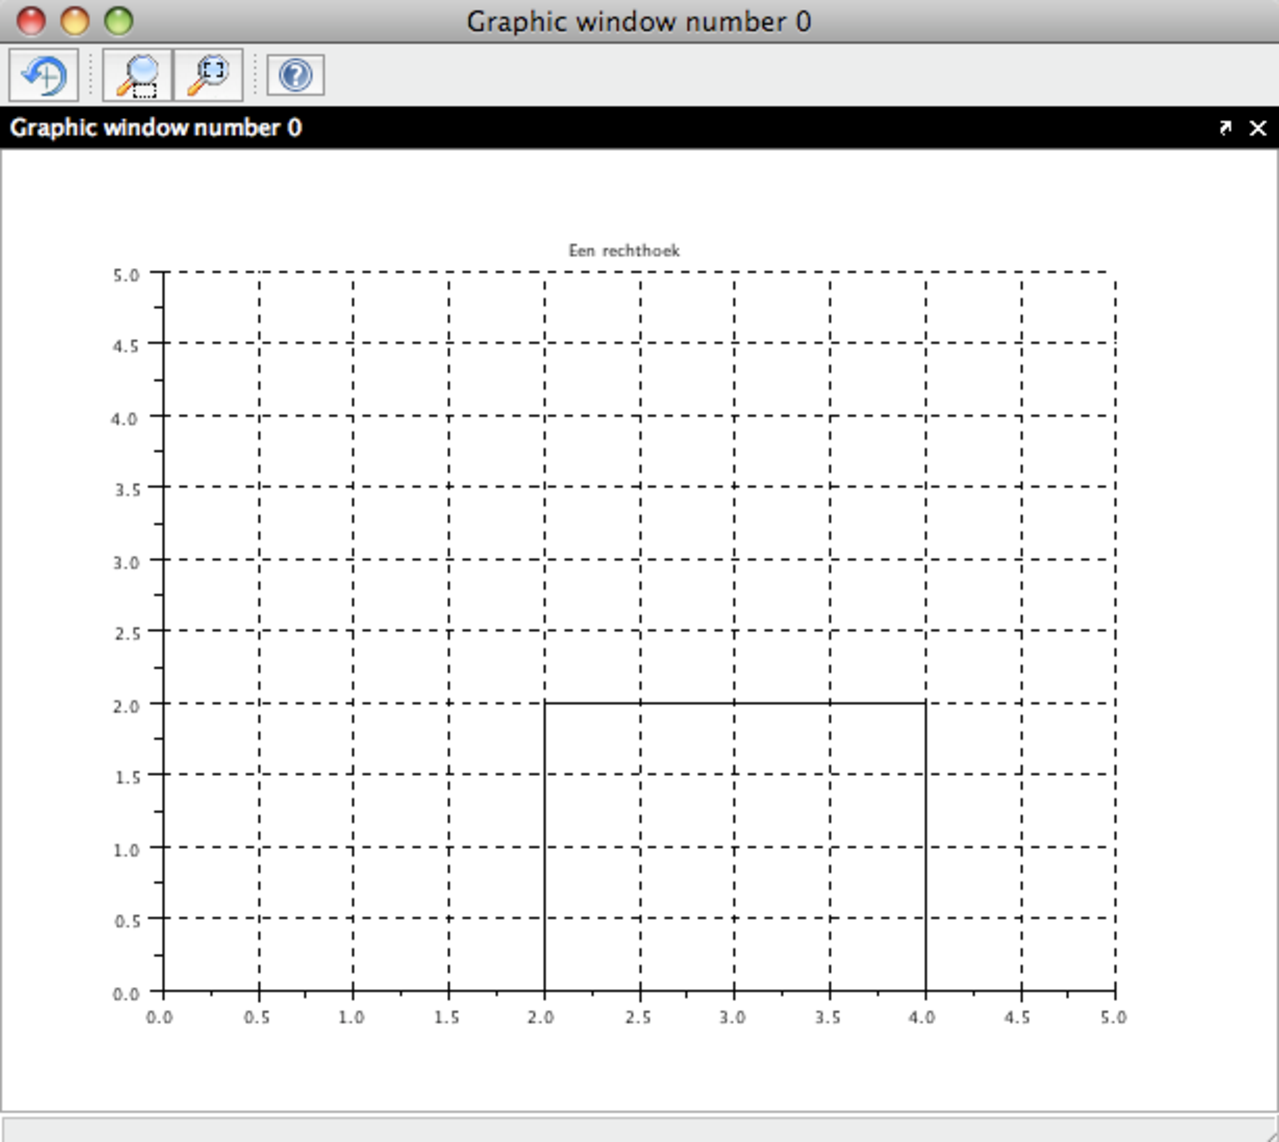
\includegraphics[width=0.8\textwidth]{figuren/scilab/11grafiek}
    \caption{Vierkant tekenen met plot2d}
	\label{figg:vierkant}
	\end{center}
\end{figure}

Scilab voorziet eindeloos veel mogelijkheden om figuren aan te passen en leesbaarder te maken met kleurtjes en titels. Typ bijvoorbeeld \verb+help plot2d+ of \verb+help gda+ in de prompt en bekijk de voorbeelden die de helpfunctie geeft.
 
 We vermelden tenslotten de functie \verb/xclick()/. Als je dit commando in de prompt ingeeft, kan je op een plaats in de grafiek klikken. Het resultaat bestaat uit drie getallen. Het eerste geeft aan met welke muisknop je geklikt hebt. De twee andere getallen geven de coördinaten aan van het punt waarop je geklikt hebt.

\section{Programmeren in Scilab}
\subsection{Functies}

We spreken over \emph{programma's}, maar eigenlijk is dat geen correcte term. In Scilab maak je nieuwe \emph{functies}. Het equivalent in Java is een \emph{methode}. 

Een functie heeft een \emph{functienaam}, een \emph{(aantal) argument(en)}, ook wel gekend als \emph{parameter(s)} en een \emph{functiedefinitie}. Elke functie heeft juist \'e\'en resultaat (zoals we later gaan zien kan dit resultaat wel bestaan uit meerdere getallen). In 
sectie~\ref{sec:werken_met_functies} vermeldden we reeds hoe je functies definieert en oproept in Scilab.


Het is belangrijk dat je de functies voldoende documenteert. Documentatie voer je in na \verb+//+. Tekst rechts hiervan wordt niet gelezen. 

\begin{lstlisting}[caption={Elke functie bevat enkele regels uitleg!}, label=Maal.sci]
function y=maal(a,b)
// deze functie berekent a*b
//
//Input Arguments:
//  a           een integer; de eerste factor
//  b           een integer; de tweede factor

y=a*b
endfunction
\end{lstlisting}

Als je een boodschap wil meegeven aan de gebruiker  kan dit met het \verb+disp+ commando. Het gebruik: \verb+disp("foutmelding")+. In listing~\ref{fac} vind je een voorbeeld. Met het commando \verb+abort+ beëindig je het programma. Je kan beide commando's samen ook vervangen door de functie \verb/error("message")/. Het programma toont de foutboodschap en keert terug naar de prompt. 


\subsection{Lussen: while en for}
De twee voornaamste lussoorten zijn 
\verb+while+ en \verb+for+. Met het sleutelwoord \verb+break+ ga je uit de lus, bijvoorbeeld wanneer je na een controle met een \verb+if+ het resultaat bekomen hebt dat je wou. Probeer het gebruik van \verb/break/ wel te vermijden, want dat geeft al snel aanleiding tot `spaghetticode'. Meestal kan het vervangen worden door een doordacht gebruik van een \verb/while/-lus.

\begin{lstlisting}[caption={Eenvoudig voorbeeld van een whilelus}, label=simpele while]
function y=testwhile(x)
  // toon de waarden van 1 t.e.m. x op het scherm
  // x moet groter of gelijk aan 1 zijn
  y=1;
  disp(y) 		// toon de waarde van y op het scherm
  while y<x
    y=y+1;
    disp(y)
  end
endfunction
\end{lstlisting}

Vorig voorbeeld is nogal eenvoudig maar het toont wel hoe een whilelus in elkaar zit. Je moet eerst de variabele $y$ initialiseren; je geeft de conditie aan van de lus. Binnen de lus geef je aan wat er moet gebeuren, en belangrijk, $y$ moet opgehoogd worden. Anders zit je met een \emph{oneindige lus}.

Een volgend voorbeeld gaat over de \verb+for+-lus.

\begin{lstlisting}[caption={Eenvoudig voorbeeld van een for-lus}, label=simpele for]
function y=testfor(x)
  // zelfde als hierboven, maar met for-lus
  
  for y=1:x
    disp(y)
  end
endfunction
\end{lstlisting}

Zoals je kan zien is een \verb+for+-lus gelijkaardig aan de \verb+while+-lus. Er zijn echter een aantal verschillen. Zo kan de variabele $y$ ge\"initialiseerd worden binnen de \verb+for+ zelf met \verb+y=1+. De conditie is ook anders dan in de while. In de for gebruik je `:' wat zo veel wil zeggen als `tot'. Je zegt dus eigenlijk dat $y$ gaat van 1 tot x. In de lus zelf mag $y$ niet opgehoogd worden: dit gebeurt door de \verb+for+-lus zelf.

\subsection{Controlestructuren}
Scilab kent het \verb+if+-statement. Een \verb+if+-statement wordt afgesloten d.m.v.\ een \verb+end+. If-statements kunnen ook genest worden. Het woordje \verb+then+ is optioneel. Als je het schrijft, moet het op dezelfde regel als de \verb+if+ staan.

\begin{lstlisting}[caption={Geneste if}, label=geneste if]
function y=verwerk(x)

if modulo(x,2) == 0
  if x==2
    y = 1
  elseif x == 4
    y = 2
  else
    y = 0
   
  end
  
elseif modulo(x,3) == 0
  y = 0
else
  y = -1
end

endfunction
\end{lstlisting}

Je merkt dat \verb+if+ afgesloten wordt met \verb+end+. Tussen
begin en einde kan je de nodige bewerkingen uitvoeren.

Er bestaan twee mogelijkheden om een alternatief te laten
uitvoeren. Als er maar \'e\'en alternatief is, gebruik je
\verb+else+. Indien er verschillende alternatieven zijn (bvb.\  $x>0$ en $x=0$), kan je \verb+elseif+ gebruiken.
Achter \verb+elseif+ typ je de te controleren voorwaarde en
vervolgens de bewerkingen indien aan de voorwaarde voldaan is.
Merk op dat \verb+elseif+ \emph{niet} afgesloten wordt met
\verb+end+.

In tabel~\ref{operatoren-scilab} vind je de belangrijkste logische
operatoren. De {\sc en}- en {\sc of}-operator heeft voorrang op de andere operatoren. Vergeet dus geen haakjes te plaatsen, bvb.\ \verb/(x>3)&(x<5)/. Let ook op het verschil tussen de \emph{toekenningsoperator} \verb+a=b+ en de \emph{logische operator} \verb+a==b+.

\begin{table}[htbp]
\centering
\caption{Logische operatoren in Scilab}
\begin{tabular}{ll}
\toprule

             & Scilab \\ 
\midrule
{\sc en, of, niet} &\verb/ &, |, ~/ \\ 
$\neq,~=$ & \verb/<>, ==/ \\ 
$<,~>,~\leq,~\geq$    & \verb/<, >, <=, >=/ \\ 
{\sc true, false}&\verb+%T, %F+\\ 
\bottomrule
\end{tabular}
 \label{operatoren-scilab}
\end{table}




\subsection{Programmeren met vectoren}

Binnen een lus kan je bewerkingen doen op ieder vectorelement. Eerst moet de vector gedefinieerd zijn. Dit kan met de functie \verb+zeros(1,n)+ waarbij \verb+n+ op voorhand moet ingevuld zijn. Onderstaand programma berekent de faculteit van de getallen 1 t.e.m. \verb+n+. Het resultaat is een vector $V_{i} = i!$.

\begin{lstlisting}[caption={Bereken faculteit van 1 t.e.m. x}, label=fac]
function V=facvector(x)
// bereken faculteit van 1 t.e.m. x
 
 if x<0; 
   disp("faculteit van negatief getal bestaat niet: 
   	de input is "+string(x))
    abort 
 // foutmelding
  else
    V=zeros(1,x); // vector definieren
    V(1)=1;       // fac(1)=1
    for i= 2 : x
      V(i)=V(i-1)*i;
    end
  end;
endfunction
\end{lstlisting}

Volgend programma berekent het grootste element van een vector:

\begin{lstlisting}[caption={Maximum van een vector}, label=maximum]
function y=maximum(V)
// berekent het grootste getal van de vector V
y=V(1);
for i=2 : length(V)
  if V(i)>y
    y=V(i)
  end
end
endfunction
\end{lstlisting}

In listing~\ref{fac} initialiseren we de vector $V$ met de functie \verb/zeros()/. Dat is enkel mogelijk als het aantal elementen van de resulterende vector gekend is. Als dat niet zo is, moet de vector $V$ geïnitialiseerd worden als een lege vector. Nadien worden de elementen één na één toegevoegd. Als voorbeeld schrijven we de functie \verb/cijfers(V)/. Input is de vector \verb+V+ van willekeurige lengte die de cijfers 0 tot en met 9 bevat. Output is een vector die alle cijfers die voorkomen in \verb/V/ juist één keer bevat van klein naar groot.
Dit wordt getoond in voorbeeld listing~\ref{lege_vector}.

\begin{lstlisting}[caption={Een vector aanmaken gedurende de functie}, label=lege_vector]
function W=cijfers(V)
  // output initialiseren
  W=[];
  // controleren of V enkel cijfers 0:9 bevat
  for i=1:length(V)
    if (V(i)<0)|(V(i)>9)
      disp('input mag enkel cijfers tussen 0 en 9 bevatten')
      abort // foute input, dus functie afbreken
    end
  end
  // cijfer per cijfer controleren of het voorkomt in V
  for i=0:9
    for j=1:length(V)
      if V(j)==i
        W=[W,i] // cijfer komt voor, dus plakken aan output-vector
        break // cijfer is gevonden, dus niet meer verder zoeken
        // voor dit cijfer
      end
    end
  end
endfunction
\end{lstlisting}

\subsection{Meerdere waarden als resultaat van een functie}
Een functie heeft steeds \'e\'en resultaat maar dit resultaat mag ook \emph samengesteld zijn uit verschillende getallen, zoals een vector. Een volgend voorbeeld zoekt zowel naar het kleinste als het grootste getal in een vector.

\begin{lstlisting}[caption={Minimum en maximum van een vector}, label=minenmax]
function [minim,maxim]=extrema(V)
// berekent het kleinste en het grootste getal 
// van de vector V
maxim=V(1);
minim=V(1);
for i=2 : length(V)
  if V(i)>maxim
    maxim=V(i);
  end;
  if V(i)<minim
    minim=V(i);
  end
end
endfunction
\end{lstlisting}

We laden de functie in in Scilab en bekijken het resultaat:

\begin{lstlisting}[caption={Het minimum en maximum in het console venster}, label=minenmaxinscilex]
-->V=[1,2,3,5,3,9,6];

-->[mi,ma] = extrema(V)
  ma =
     
     9.
  mi =

     1.
\end{lstlisting}

Aangezien de functie als resultaat een lijst met twee waarden geeft moet je de functieoproep gelijkstellen aan een lijst met twee variabelen (hier mi en ma). Er is echter nog een andere mogelijkheid om een resultaat van meerdere getallen te bekomen: een \emph{vector} of een \emph{matrix}. Dit wordt gedemonstreerd in een volgend voorbeeld.

\begin{lstlisting}[caption={Functie euro(x)}, label=euro]
function G=euro(x)
// berekent het aantal briefjes en stukken om een
// bedrag x in euro te vormen met zo weinig mogelijk
// briefjes of stukken
E=[500,200,100,50,20,10,5,2,1,0.50,0.20,0.10,0.05,0.02,0.01];
G=zeros(size(E));
for i=1 : length(E)
  G(i)=floor(x/E(i));
  x=x-G(i)*E(i);
  if G(i) ~= 0
    disp([E(i),G(i)]) // Uitvoer naar het scherm
  end
end
endfunction
\end{lstlisting}

Deze functie geeft soms echter fouten. Waarom denk je?

%\end{document}
\section{Oefeningen}
\begin{oef}
   Bereken volgende uitdrukkingen in SciLab: 
\begin{enumerate}
\item  $\dfrac{4\cdot \pi-7}4 \cdot 2+10$
\item $\dfrac{ -7^3}8 $
\item $| - 4| $
\item mod(7, 3), mod($ -15$, 4) 
\item floor($-2.45$) 
\item $500\cdot 1.05^\frac{12}2\cdot \dfrac{1-1.05^\frac{-13}2}{1-1.05^\frac{-1}2} $
\end{enumerate}
   \begin{opl}
\begin{enumerate}
\item  12.783185	
\item - 42.875
\item 4
\item 1, -3 
\item -3
\item 7555.9475
\end{enumerate}
   \end{opl}
\end{oef}

\begin{oef}
Definieer de functie $opp(z)$ die de totale oppervlakte berekent 
van een kubus met zijde $z$. Bereken nu de oppervlakte 
als $z$ gelijk is aan \num{2.5} of \num{3.125}. 
\end{oef}

\begin{oef}
      Een rol behangpapier is \SI{10}{\meter} lang. Stel de veranderlijke  $t$ gelijk aan de hoeveelheid behangpapier die je nodig hebt, uitgedrukt in meter. Stel \verb/aantalrollen/ het aantal rollen dat je moet kopen om aan de  hoeveelheid $t$ te voldoen. Teken de grafiek van de functie \verb/aantalrollen/.
\end{oef}


\begin{oef}
De studentenkring organiseert een voetbalwedstrijd. De materiaalmeester heeft \SI{100}{\meter} lint bij om het voetbalterrein af te spannen. 
\begin{enumerate}
\item Teken de grafiek van de functie \verb/breedte/ die de breedte $b$ van het terrein in functie van de lengte $l$ weergeeft.
\item Teken de grafiek van de functie \verb/opp/ die de oppervlakte $o$ van het terrein in functie van de lengte $l$ weergeeft. Voor welke lengte is de oppervlakte maximaal?
\end{enumerate}
\end{oef}

\begin{oef}
(Moeilijker) Er is een misdaad gebeurd. De politie moet twee oppervlakten afspannen. Ze gebruikt daarvoor \SI{60}{\meter} lint. De eerste oppervlakte is cirkelvormig. De tweede oppervlakte is een vierkante oppervlakte die langs \'e\'en zijde aan een muur grenst. Langs de muur hoeft geen lint gespannen te worden. 
\begin{enumerate}
\item Definieer de functie \verb/oppervlakte/ die de afgespannen oppervlakte $opp$ toont in functie van zijde $z$ van het vierkant.
\item Teken deze functie.
\item Wat zijn de afmetingen van cirkel en vierkant opdat de afgespannen oppervlakte minimaal is?
\end{enumerate}
\end{oef}

\begin{oef}
Teken de functies $y = 5^x$ en $y = \frac15^x$
op hetzelfde scherm. 
Zorg voor aangepast bereik van de co\"ordinaatassen. Verzorg ook de titel van de grafiek.
\end{oef} 


\begin{oef}
Herschrijf de functie van listing~\ref{fac} waarbij je te werk gaat zoals in listing~\ref{lege_vector}.
\end{oef}

\begin{oef}
    Schrijf de functie  \verb/sommeetk(a,r,n)/, 
    die de som berekent van opeenvolgende elementen van een meetkundige rij. De veranderlijke  $a$ is de 
    eerste term van de som, $v$ is de reden van de meetkundige rij en de som 
    bevat $n$ termen. Geef als output  de som en de laatste term van de som.
    (meervoudige output). Gebruik eerst de \verb/for/-lus , daarna  de \verb/while/-lus.
    \end{oef} 



\begin{oef}
Definieer in Scilab volgende matrices en vectoren:
\begin{enumerate}
\item $\displaystyle 
	A=\begin{bmatrix}1&2&3\\4&5&6\\7&8&9\end{bmatrix}$
\item $B=\begin{bmatrix}1&2&3&4&\ldots&19&20\end{bmatrix}$
\item $C=\begin{bmatrix}1\\2\\3\\ \ldots \\19\\20\end{bmatrix}$
\item $D=\begin{bmatrix}2\\4\\6\\\ldots\\38\\40\end{bmatrix}$
\end{enumerate}
\end{oef}


\begin{oef}
Bepaal het element van $A$ op de tweede rij, derde kolom.
\end{oef}
\begin{oef}
Definieer de submatrix $E$ die bestaat uit de eerste 5 kolommen van $B$.
\end{oef}
\begin{oef}
Voeg de matrices $C$ en $D$ samen tot een matrix met 2 kolommen en 20 rijen.
\end{oef}

\begin{oef}
Schrijf de functie \texttt{vermenigvuldigMatrix(M,a)} die elk element van de matrix $M$ vermenigvuldigt met $a$.
\end{oef}
\begin{oef}
Schrijf de functie \texttt{kolomNaarRij(V)} die de kolomvector $V$ herschrijft tot een rijvector.
\end{oef}
\begin{oef}
Schrijf de functie \texttt{keerOm(V)} die de rijvector $V$ ``omkeert'': eerste element wordt het laatste enz.
\begin{opl}Eén van de vele mogelijke oplossingen:
\begin{lstlisting}[caption={Een vector omkeren}, label=vectoromkeren]
function W=keerom(V)
  // schrijft vector V in omgekeerde volgorde
  W=V
  l=length(V)
  for i=1:l
    W(l+1-i)=V(i)
  end
endfunction
\end{lstlisting}
\end{opl}
\end{oef}
\begin{oef}
Schrijf de functie \texttt{maakMatrix(n)} die een vierkante matrix met $n$ e\-le\-menten genereert. Indien $n$ geen kwadraat is van een geheel getal, toont de functie een foutboodschap en geeft ze {\sc false} (\texttt{\%F}) terug.
\end{oef}
   
\begin{oef}
   Schrijf de functie \func{aantal(K,r,T)}, die volgend probleem oplost:
   \begin{quote}
     Er staat nu \euro $K$  op een rekening met  rente $r$  per periode.
Elke periode wordt er \euro ${T}$ van de  rekening afgehaald. 
Na 1 periode haal je voor de eerste keer \euro ${T}$ af.
\begin{enumerate}
    \item  Zoek hoeveel keren 
je het bedrag $T$ kan afhalen zonder dat de rekening in onder nul komt.


    \item Als output geef je het aantal keren dat je een bedrag 
    $T$ afhaalde en het bedrag dat nog op de rekening overblijft na 
    de laatste $T$ af te halen.
\end{enumerate}  
   \end{quote}
   \end{oef}

\begin{oef}
Schrijf de functie \func{posnegvector(n)} die een vector $V$ 
weergeeft met hoogstens $n$ elementen. In het programma wordt hoogstens $n$ keren 
een geheel getal opgevraagd (gebruik het commando \emph{a=input(`  \ldots')}):
indien dit getal positief is geef je  het element van de vector de waarde 1, 
indien het getal negatief is dan wordt het element van de vector gelijk aan -1.
De vector eindigt als de opgevraagde input =0.
\end{oef}
\begin{oef}
Definieer de samengestelde functie \func{g(x)} met
    als voorschrift:
$g(x)=2*x-3$ als $x<2$ en $g(x)=(x-3)+2$ als $x>=2$. 
Teken die functie op het
interval $[-5,5]$.
\end{oef}

\begin{oef}
    Schrijf de functie \func{zoekdelers(x,v),} met $x$ een 
    geheel getal kleiner dan  $10000$, en $V$, een vector met een 
    aantal priemgetallen. De output van de functie is een nieuwe 
    vector $W$ die alleen die priemgetallen uit $V$ bevat die deler 
    zijn van $x$.\\
    \textbf{Uitbreiding} De output is nu een matrix met 2 rijen. De 
    eerste rij is de vector $W$ zoals hierboven vermeld. De tweede 
    rij geeft voor elke priemdeler uit $W$ aan, hoe dikwijls die voorkomt in 
    de ontbinding van $x$.
    \end{oef}
\begin{oef}
Het algoritme van Euclides dient  om de grootste gemene delers van 2 gehele getallen
te vinden. Zoek het algoritme op op internet. Schrijf nu de functie 
\func{ggd(D,d)} die dit algoritme toepast en als output de grootste gemene deler van de gehele getallen \verb+D+ en \verb+d+ weergeeft.
\end{oef}

\begin{oef}
Schrijf de functie \func{reverse(V)}, met output de vector $W$ 
waarbij de elementen van $V$ in omgekeerde volgorde voorkomen.\\
\textbf{Uitbreiding  \func{reverse(V,n})}. De elementen van $V$ 
moeten niet alleen in omgekeerde volgorde voorkomen maar elk element 
moet $n$ keren herhaald worden.
\end{oef}

\begin{oef}
Schrijf drie verschillende functies die de matrix 
\begin{equation*}
\begin{bmatrix}
 1&2  &3  \\
 4& 5 &6 \\
 7& 8 &9
\end{bmatrix}
\end{equation*}
genereren. Input is de integer \verb+n+. Als \verb+n+ geen kwadraat is, genereert de functie een foutmelding.
\end{oef}

\begin{oef}
Kerstmis 2003 kochten we een kerstboom van \SI{1}{\meter}. Nadien plantten we hem in de tuin. Hij groeit jaarlijks \SI{30}{\centi\meter}. Met Kerstmis zetten we hem elk jaar weer binnen. Onze living is \SI{2,30}{\meter} hoog. Tot welk jaar kunnen wij onze kerstboom gebruiken zonder er een stukje af te moeten snijden? Schrijf de functie \verb/y=kerstboom()/ die volgende boodschap doet verschijnen op het scherm: ``Met kerstmis in het jaar y zult u een nieuwe kerstboom moeten kopen.'' Vervang \verb/y/ door het berekende jaartal.
\end{oef}



\begin{oef}
Schrjif de functie \verb/EuroNaarEurocent(V)/. Input is de vector \verb/V/ met twee elementen (aantal euro, aantal eurocent). Output is het totaal aantal eurocent.
\end{oef}
\begin{oef}
Schrijf de functie \verb/EurocentNaarEuro(x)/ die het omgekeerde doet van de vorige functie.
\item Schrijf de functie \verb/GeefTerug(V,W)/. Input is het bedrag dat overhandigd werd, genoteerd door de vector \verb/V/ (euros en eurocenten), en het bedrag dat moet betaald worden, eveneens als vector.
\end{oef}
\begin{oef}
Schrijf de functie \verb/MaxSom(V)/. Input is de vector \verb/V/. Output is de positie van de grootste som van 3 opeenvolgende elementen (begin- en eindindex) én de waarde van die som. Test de functie ook met negatieve getallen!
\end{oef}
\begin{oef}
Schrijf de functie \verb/gemiddelde(V)/: output is het gemiddelde van de vector \verb/V/.
\end{oef}
\begin{oef}
Schrijf de functie \verb/aantalElementenGroterDanGemiddelde(V)/: input vector \verb/V/, output aantal elementen van \verb/V/ die groter zijn dan het gemiddelde van de elementen van \verb/V/.
\end{oef}
\begin{oef}
Schrijf de functie \verb/ElementenGroterDanGemiddelde(V)/. Output is de vector \verb/W/ die alle elementen bevat die groter zijn dan het gemiddelde van \verb/V/. Breid daarna uit naar een matrix.
\end{oef}
\begin{oef}
Schrijf de functie \verb/equals(V,W)/ die controleert of de vectoren \verb/V/ en \verb/W/ gelijk zijn aan mekaar.
\end{oef}
\begin{oef}
Schrijf de functie \verb/equalsMatrix(M,N)/ die controleert of de matrices \verb/M/ en \verb/N/ gelijk zijn aan mekaar.
\end{oef}








